\documentclass[journal=nalefd,manuscript=letter,layout=traditional]{achemso}

\usepackage{amsmath}
\usepackage{graphicx}
\usepackage{microtype}
\usepackage{siunitx}
\usepackage{booktabs}
\usepackage{bm}
\usepackage{xr}
\usepackage[hidelinks]{hyperref}
% Figure references.  Every figure number in this project is produced by
% \ref, never typed by hand: \ref{fig:...} for figures of this document, and
% \ref{SI-fig:...} for figures of the other one, whose labels the xr package reads
% out of its .aux.  Panel letters are appended literally, e.g.
% Figure~\ref{fig:xpcs}a.  `make papers` compiles si -> main -> si so both
% directions resolve on a clean tree; `make check` reports any that did not.
\externaldocument[SI-]{build/si}

% Line numbers, for the reviewers' convenience.  lineno does not see amsmath's
% display environments by itself, so a numbered equation would silently break
% the count; \linenoAms wraps them in \linenomath, which is the standard fix.
\usepackage[mathlines]{lineno}
\linenumbers
\newcommand*\linenoAms[1]{%
  \expandafter\let\csname old#1\expandafter\endcsname\csname #1\endcsname
  \expandafter\let\csname oldend#1\expandafter\endcsname\csname end#1\endcsname
  \renewenvironment{#1}{\linenomath\csname old#1\endcsname}%
                       {\csname oldend#1\endcsname\endlinenomath}}
\AtBeginDocument{\linenoAms{equation}\linenoAms{equation*}%
                 \linenoAms{align}\linenoAms{align*}}

\setkeys{acs}{articletitle=true}
\SectionNumbersOff
\graphicspath{{figures/}}
\sisetup{detect-all=true,range-phrase=--,range-units=single}

\newcommand{\VPAVG}{(VPAVG)$_{30}$}
\newcommand{\Ainv}{\text{\AA}$^{-1}$}

% Data-derived figures are drawn at exactly the ACS column widths (3.33 in
% single, 7.0 in double), so they are included at NATURAL SIZE -- no width=
% scaling -- and the 8 pt lettering in the file is 8 pt on the page.  A
% double-column figure is wider than this class's 6.52 in text block, so
% \makebox lets it overhang symmetrically into the margins instead of being
% shrunk.  Setup.pdf is the approved original artwork and is not on that grid,
% so it keeps width=\linewidth.
\newcommand{\acsfig}[1]{\makebox[\linewidth][c]{\includegraphics{#1}}}

\title{Reversible $\beta$-Sheet-like Ordering and XPCS-Resolved Dynamic Arrest during Elastin-like Polypeptide Phase Separation}

\author{Doga Ozgulbas}
\affiliation{Data Science and Learning Division, Argonne National Laboratory, Lemont, Illinois 60439, United States}
\author{Miaoqi Chu}
\affiliation{X-ray Science Division, Argonne National Laboratory, Lemont, Illinois 60439, United States}
\author{Alex Lavens}
\affiliation{Data Science and Learning Division, Argonne National Laboratory, Lemont, Illinois 60439, United States}
\author{Nicholas Marks}
\affiliation{Data Science and Learning Division, Argonne National Laboratory, Lemont, Illinois 60439, United States}
\author{Ming Du}
\affiliation{X-ray Science Division, Argonne National Laboratory, Lemont, Illinois 60439, United States}
\author{Xiaobing Zuo}
\affiliation{X-ray Science Division, Argonne National Laboratory, Lemont, Illinois 60439, United States}
\author{Michael Irvin}
\affiliation{Data Science and Learning Division, Argonne National Laboratory, Lemont, Illinois 60439, United States}
\author{Heng Ma}
\affiliation{Data Science and Learning Division, Argonne National Laboratory, Lemont, Illinois 60439, United States}
\author{Soenke Seifert}
\affiliation{X-ray Science Division, Argonne National Laboratory, Lemont, Illinois 60439, United States}
\author{Byeongdu Lee}
\affiliation{X-ray Science Division, Argonne National Laboratory, Lemont, Illinois 60439, United States}
\author{Rafael Vescovi}
\affiliation{Data Science and Learning Division, Argonne National Laboratory, Lemont, Illinois 60439, United States}
\author{Ian Foster}
\affiliation{Data Science and Learning Division, Argonne National Laboratory, Lemont, Illinois 60439, United States}
\author{Victor Mateevitsi}
\affiliation{Argonne Leadership Computing Facility, Argonne National Laboratory, Lemont, Illinois 60439, United States}
\author{Don Jensen Jr.}
\affiliation{X-ray Science Division, Argonne National Laboratory, Lemont, Illinois 60439, United States}
\author{Arvind Ramanathan}
\email{ramanathana@anl.gov}
\affiliation{Data Science and Learning Division, Argonne National Laboratory, Lemont, Illinois 60439, United States}
\author{Chase Akins}
\affiliation{Biosciences Division, Argonne National Laboratory, Lemont, Illinois 60439, United States}
\author{Gyorgy Babnigg}
\email{gbabnigg@anl.gov}
\affiliation{Biosciences Division, Argonne National Laboratory, Lemont, Illinois 60439, United States}
\author{Qingteng Zhang}
\email{qzhang234@anl.gov}
\affiliation{X-ray Science Division, Argonne National Laboratory, Lemont, Illinois 60439, United States}

\begin{document}

\begin{abstract}
Amyloid-like $\beta$-sheet order is usually associated with persistent aggregates, yet related contacts can also act as reversible physical junctions. Temperature-dependent SAXS/WAXS of sequence-defined \VPAVG{} reveals a reversible transition from a molecularly dispersed state at \SI{10}{\degreeCelsius} to a hierarchical assembly at \SI{30}{\degreeCelsius}, with an approximate $I(Q)\propto Q^{-3.2}$ low-$Q$ response and peaks at $Q=1.38$ and $0.72$~\Ainv, compatible with $\beta$-sheet-like packing. In a separate isothermal experiment on a freshly loaded sample, SA-XPCS at \SI{30}{\degreeCelsius} shows a two-step correlation decay whose fast-decay amplitude falls progressively across \SIrange{76}{167}{\nano\meter} over \SI{47}{\minute}, indicating an increasing fraction of the scattering ensemble is arrested within the \SI{1.6}{\second} maximum accessible delay. Thermally reversible $\beta$-sheet-like local order therefore coexists with progressive mesoscale arrest, indicating that amyloid-like packing need not imply irreversible aggregation and offering a route to thermally switchable protein networks.
\end{abstract}

Amyloid-like $\beta$-sheet ordering occupies an unusual position in protein science and polymer materials. Pathological amyloid fibrils formed by unrelated proteins and peptides are associated with Alzheimer’s disease,\cite{Masters1985-pnas} Parkinson’s disease,\cite{Serpell2000-pnas} type II diabetes,\cite{Cooper1987-pnas} prion diseases,\cite{Pan1993-pnas} and systemic light-chain amyloidosis.\cite{Radamaker2019-ncomms} Many amyloid fibrils are kinetically persistent because extended hydrogen-bonded sheets are reinforced by tightly packed steric-zipper interfaces.\cite{Sawaya2007-nature} Yet amyloid-like order is not intrinsically pathological: functional amyloids store mammalian peptide hormones in pituitary secretory granules\cite{Maji2009-science} and build the extracellular matrix of bacterial biofilms,\cite{Chapman2002-science} and related assemblies are increasingly used as mechanically robust biomaterials.\cite{Knowles2016-am} What differs across these systems is not whether $\beta$-sheet-like order forms but how long it lasts: hormone granules disassemble to release functional monomer, whereas steric-zipper cores are far more persistent. Amyloid-like packing therefore spans a wide range of stabilities rather than committing a sequence to one permanent structure,\cite{Palmadottir2025-bpr} and where a sequence falls in that range is a materials-design variable.

Reversible $\beta$-sheet-like contacts are attractive as candidate physical junctions because backbone hydrogen bonding can stabilize locally ordered assemblies, whereas hydrated or weakly packed interfaces can remain dynamic or reversible.\cite{Kato2012-cell,Hughes2018-science,Luo2018-nsmb,Palmadottir2025-bpr} Elastin-like polypeptides (ELPs) are well suited to test this possibility because their sequence, molecular weight, and lower critical solution temperature (LCST) behavior can be programmed recombinantly.\cite{Meyer2004-zb,Amiram2011-la,Quiroz2015-mh,Varanko2020-ek,Saha2020-jg} Above the LCST, ELPs undergo hydrophobic desolvation and can form coacervates or hierarchical assemblies depending on sequence, concentration, and thermal history.\cite{Varanko2020-ek,Saha2020-jg,Sing2017-zq} In particular, alanine-containing ELPs can form stiff, thermoresponsive gels through arrested phase separation.\cite{Glassman2015-cw,Glassman2016-pq} Building on that work, the complementary question addressed here is whether local $\beta$-sheet-like packing can emerge reversibly while the mesoscale assembly progressively loses mobility.

Resolving whether a structurally assembled state remains dynamically evolving requires a dynamical measurement. In colloidal gels, microscopic relaxation can continue to evolve after the time-averaged structure changes only weakly, a nonequilibrium process commonly termed physical aging.\cite{Bahadur2019-ln,Chen2023-ho} Related heterogeneous relaxation has been resolved during protein liquid--liquid phase separation,\cite{Girelli2021-zz} protein gelation,\cite{Begam2021-fh} and cage relaxation in crowded protein solutions.\cite{Chushkin2022-bw} During arrested phase separation, a protein-rich morphology can therefore continue to reorganize through junction exchange, stress relaxation, and residual coarsening even when its SAXS profile changes modestly. SA-XPCS probes that evolution directly through speckle decorrelation at the same low-$Q$ length scales sampled by SAXS.

Here, temperature-dependent SAXS/WAXS and isothermal SA-XPCS provide complementary structural and dynamical views of concentrated aqueous \VPAVG. At \SI{10}{\degreeCelsius} the scattering is dominated by molecular dimensions with no detectable mesoscale assembly; heating to \SI{30}{\degreeCelsius} produces hierarchical low-$Q$ scattering and high-$Q$ peaks compatible with $\beta$-sheet-like packing, and cooling restores the low-temperature profile. In a separate experiment on a freshly loaded sample, isothermal SA-XPCS at \SI{30}{\degreeCelsius} reveals a two-step decay whose fast fraction falls progressively with elapsed time. The central result is therefore a reversible structural transition coexisting with a time-dependent loss of mesoscale mobility.

Figure~\ref{fig:setup} summarizes the SA-XPCS experiment. Its upper-left cartoon illustrates one candidate pathway, not a direct observation: protein-poor solvent regions are hypothesized to appear and grow within the slower protein-rich phase, displacing and compressing it toward a coarsened, network-like morphology. This dynamic-asymmetry picture follows Tanaka's viscoelastic phase-separation framework and is consistent with prior scattering studies of arrested ELP gels.\cite{Tanaka2000-qq,Glassman2015-cw} The \VPAVG{} sample (approximately \SI{100}{\milli\gram\per\milli\liter}) contained \SI{20}{\milli\mole\per\liter} HEPES (pH 8), \SI{250}{\milli\mole\per\liter} NaCl, and \SI{2}{\milli\mole\per\liter} DTT. Each \SI{2}{\second} SA-XPCS acquisition at APS 8-ID-I (Experimental Section) used a previously unexposed sample position; temporal and azimuthal averaging yielded $I(Q)$ and multi-tau correlation analysis yielded $g_2(Q,\Delta t)$.

\begin{figure}[htbp]
  \centering
  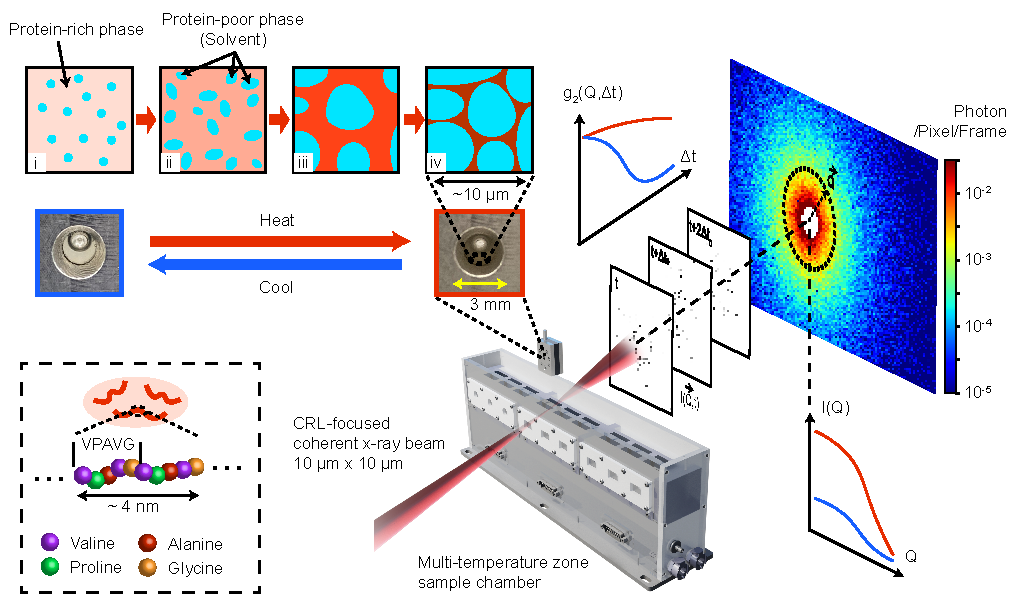
\includegraphics[width=\linewidth]{Setup.pdf}
  \caption{SA-XPCS measurement of thermally induced \VPAVG{} assembly at APS 8-ID-I. Each 100,000-frame set of sparse \SI{20}{\micro\second} frames feeds two analyses. Averaging them in time gives the SAXS intensity $I(Q)$: how much structure the sample has at each length scale $2\pi/Q$, which grows at low $Q$ on heating. Correlating them in time gives $g_2(Q,\Delta t)$: how fast the structure at that same length scale rearranges. A temporal decay in $g_2$ meaning the density fluctuations at $2\pi/Q$ are still moving, and a flat $g_2$ that they are frozen over the accessible delay times $\Delta t$. Both are sketched beside the detector (red: assembled; blue: dispersed; illustrative, not data). Center: the aluminum cell, liquid chamber \SI{3}{\milli\meter} across. The photos show the ELP samples below and above the transition (blue and red countor, respectively). Lower left: one \VPAVG{} repeat, residues colored as keyed. Right: the frame-averaged detector image, color bar in photons per pixel per frame, white center the beamstop mask; the graininess is sparse counting statistics, not resolved speckle. Upper left, stages i--iv: a conceptual illustration of the viscoelastic phase-separation pathway,\cite{Tanaka2000-qq,Glassman2015-cw} in which protein-poor solvent pools (cyan) nucleate and grow within the still-continuous protein-rich phase (deepening red: more protein), coarsening it toward a network-like morphology.}
  \label{fig:setup}
\end{figure}

Figure~\ref{fig:static} establishes the low- and high-temperature structures and their reversibility. Two aliquots from the same stock were sealed in \SI{2}{\milli\meter} quartz capillaries and measured at APS 12-ID-B using simultaneous SAXS/WAXS detection at \SI{13.3}{\kilo\electronvolt}.\cite{APS12IDB,Xu2022-12IDB,Zheng2022-12IDB} The aliquot labeled ``Measurement'' had undergone more than 10 heating/cooling cycles, whereas the ``Reference'' aliquot had remained at \SI{4}{\degreeCelsius}. At \SI{10}{\degreeCelsius}, the two profiles overlap. A Guinier fit to the Reference data gives an apparent $R_g=22.65\pm0.50$~\AA{} (Figure~\ref{SI-fig:S7}), consistent with a dispersed, unassembled low-temperature state lacking detectable mesoscale aggregates; this profile is recovered after repeated cycling. The \SI{10}{\degreeCelsius} profiles span $0.0081<Q<1.41$~\Ainv{} and the \SI{30}{\degreeCelsius} profiles $0.0046<Q<1.61$~\Ainv, so the absence of mesoscale assembly at \SI{10}{\degreeCelsius} is established for structures below approximately \SI{78}{\nano\meter}. At \SI{30}{\degreeCelsius}, both aliquots reproducibly develop an approximate $I(Q)\propto Q^{-3.2}$ response at low $Q$ (slopes fitted over $0.012<Q<0.040$~\Ainv: $-3.17$ for the Reference and $-3.15$ for the Measurement aliquot). Both aliquots also develop the same pair of high-$Q$ features, at $Q=1.38$ and $0.72$~\Ainv{} in the Reference aliquot and 1.36 and 0.74~\Ainv{} in the Measurement aliquot. The Measurement aliquot alone makes the point for the high-$Q$ features: after more than 10 cycles it still develops both peaks at \SI{30}{\degreeCelsius} and shows neither at \SI{10}{\degreeCelsius}. Their close overlap at both temperatures shows reproducible interconversion within the sensitivity of the scattering measurements. A more direct test at 8-ID-I took one aliquot---rather than two compared to each other---through seven consecutive \SIrange{6}{34}{\degreeCelsius} cycles at \SI{1}{\degreeCelsius\per\minute} (Figure~\ref{SI-fig:S6}). Across the seven cycles the \SI{6}{\degreeCelsius} profile recovers to within a 9\% relative standard deviation with no systematic drift, and at \SI{33.8}{\degreeCelsius} the correlation function is flat at $1+\beta$ in every cycle, the signature of an arrested state. The sample therefore gelled on every heating and returned to the same low-temperature state on every cooling (SI Section~\ref{SI-sec:thermalcycling}). Video~S1 independently shows recovery of optical transparency after cooling.

\begin{figure}[htbp]
  \centering
  \acsfig{Figure2_SAXS_WAXS.pdf}
  \caption{Temperature-dependent structure and reversibility of \VPAVG. At \SI{10}{\degreeCelsius}, the Measurement and Reference profiles overlap and the Reference data give an apparent $R_g=22.65\pm0.50$~\AA{} (Figure~\ref{SI-fig:S7}). Heating produces an approximate $Q^{-3.2}$ low-$Q$ response and peaks at $Q=1.38$ and $0.72$~\Ainv, corresponding to real-space spacings of approximately 4.5 and 8.8~\AA, respectively. The dashed line is an unweighted power-law fit to the Reference profile at \SI{30}{\degreeCelsius} over $0.012<Q<0.040$~\Ainv. Inset: the high-$Q$ region of that same profile (open circles, same arbitrary intensity units as the main panel); red curves are independent Gaussian-plus-linear-background fits over $0.48<Q<1.00$ and $1.18<Q<1.70$~\Ainv, and the red dashed lines and labels mark the fitted peak centers. The recovery and reproducible re-formation of these signatures demonstrate a thermally reversible structural transition within experimental sensitivity.}
  \label{fig:static}
\end{figure}

The two reciprocal-space regimes describe a hierarchical assembly. Power-law small-angle scattering signifies self-similar density heterogeneity over the probed interval rather than a single resolved structural scale.\cite{Teixeira1988-jac} Related gel-forming ELPs exhibit disordered bicontinuous or fractal protein-rich networks produced by arrested phase separation.\cite{Glassman2015-cw,Glassman2016-pq} The 4.5 and 8.8~\AA{} spacings are compatible with strand-to-strand and sheet-to-sheet packing in cross-$\beta$-like assemblies.\cite{Sawaya2007-nature,Sunde1997-jmb} Both features are broad and exhibit full widths at half maximum of 0.25 and 0.34~\Ainv{} (correlation lengths $2\pi/\Delta Q$ of only about 25 and 19~\AA), so the ordering extends over a few repeat spacings rather than forming extended cross-$\beta$ crystallites. Their concurrent appearance with the low-$Q$ response establishes coexistence of local ordered contacts and mesoscale density heterogeneity, but does not by itself prove that the contacts are the network junctions: the same two signatures would appear if the ordered contacts sat inside the protein-rich domains rather than at the links between them, and the two $Q$ ranges cannot distinguish those cases. What the literature does establish is that contacts of this kind are capable of the role: hydrated or weakly packed $\beta$-sheet interfaces form dynamic hydrogel contacts and reversible fibrils.\cite{Kato2012-cell,Hughes2018-science,Luo2018-nsmb} The disappearance of the peaks on cooling therefore identifies thermally labile $\beta$-sheet-like associations that are plausible, rather than uniquely established, physical junctions.

To resolve the evolution at fixed thermal driving force, a freshly loaded sample was held at \SI{6}{\degreeCelsius} for more than \SI{30}{\minute}, warmed to \SI{20}{\degreeCelsius} at \SI{5}{\degreeCelsius\per\minute}, and then brought to \SI{30}{\degreeCelsius} at \SI{1}{\degreeCelsius\per\minute}, the slow final ramp limiting overshoot past the target. The waiting time $t_w$ was defined from the moment the calibrated RTD, embedded in the Peltier stage adjacent to the cell, read \SI{30}{\degreeCelsius}; that moment is also the start of the first acquisition plotted in Figure~\ref{fig:xpcs}. The sample was then followed by simultaneous SAXS and SA-XPCS for up to \SI{7863}{\second} (Figure~\ref{fig:xpcs}). Each reported $t_w$ labels a group of consecutive \SI{2}{\second} acquisitions, each at a previously unexposed position, that were averaged together, and $t_w$ is the acquisition time of the first member. The groups are not all the same size. The five analyzed for $g_2$ hold 150, 100, 100, 100 and 63 acquisitions and run 15.5, 10.4, 10.4, 10.7 and \SI{6.7}{\minute}; the last is short only because the measurement ended there. The $t_w=0$ SAXS profile of Figure~\ref{fig:xpcs}a averages the first 200 acquisitions, over \SI{20.8}{\minute}. The SAXS intensity initially lies close to the \SI{6}{\degreeCelsius} reference profile and then rises, as $t_w$ advances, by more than two orders of magnitude at low $Q$, while remaining broad and monotonic (Figure~\ref{fig:xpcs}a and Figure~\ref{SI-fig:S8}). This evolution documents increasing mesoscale density contrast without selection of a narrow domain spacing. Both the elapsed-time and the $Q$ range analyzed below are set by photon statistics rather than by a change in the sample's dynamics. Before $t_w=5039$~s the low-$Q$ coherent intensity is too weak for a two-step correlation function to be resolved above the noise. Figure~\ref{SI-fig:S6}c shows the still-mobile limit directly: at \SI{31.9}{\degreeCelsius} the correlation decays essentially to its baseline within the accessible delay range, so no second, slower step is present there to resolve. Above $Q=0.00827$~\Ainv{} the scattered intensity has fallen by more than an order of magnitude (Figure~\ref{fig:xpcs}a) and the corresponding $g_2$ is dominated by counting noise. Reliable correlation functions are therefore restricted to $t_w\ge5039$~s and the five lowest $Q$ bins.

The intensity autocorrelation function is
\begin{equation}
 g_2(Q,\Delta t)=\frac{\langle I(Q,t)I(Q,t+\Delta t)\rangle_t}{\langle I(Q,t)\rangle_t^2},
 \label{eq:g2}
\end{equation}
where $I(Q,t)$ is the coherent scattering intensity and $\Delta t$ is the delay time. Through the Siegert relation, $g_2$ reports the relaxation of density fluctuations at length scale $2\pi/Q$. At $Q=0.00376$~\Ainv{} (approximately \SI{167}{\nano\meter}), the correlation functions show a two-step decay: an initial millisecond-scale relaxation followed by an apparent plateau that persists throughout the \SI{2}{\second} acquisition (Figure~\ref{fig:xpcs}b). With increasing $t_w$, the amplitude of the first decay decreases and the plateau rises. The fraction of fast dynamics therefore decreases while the arrested fraction increases. Such two-step relaxation and growth of a slow component are characteristic of heterogeneous kinetic arrest in protein and colloidal gels.\cite{Begam2021-fh,Bahadur2019-ln,Chen2020-fn}

The correlation functions were parameterized by
\begin{equation}
 g_2(Q,\Delta t)=1+\beta\left[
 f(Q)\exp\!\left[-\left(\frac{\Delta t}{\tau_{\mathrm{fast}}(Q)}\right)^{p_{\mathrm{fast}}}\right]
 +\left[1-f(Q)\right]\exp\!\left[-\left(\frac{\Delta t}{\tau_{\mathrm{slow}}(Q)}\right)^{p_{\mathrm{slow}}}\right]
 \right]^2,
 \label{eq:twomode}
\end{equation}
where $\beta$ is the instrumental speckle contrast, measured independently on a static reference and held fixed (Figure~\ref{SI-fig:S4}), $f(Q)$ is the fitted fraction of fast dynamics, $1-f(Q)$ is the fitted fraction of slow dynamics, and $\tau_{\mathrm{fast}}(Q)$ and $\tau_{\mathrm{slow}}(Q)$ are effective relaxation times. The stretching exponents $p_{\mathrm{fast}}$ and $p_{\mathrm{slow}}$ carry no $Q$ argument because they are the shared parameters of a global fit: at each elapsed time the five measured $Q$ bins were fitted simultaneously with both exponents common to all five. Sharing them reduces the free parameters from 25 to 17 and tightens the ones that remain. Fitted this way, with the two exponents as shared global fitting parameters, the two-mode form describes the observed first decay and persistent plateau without assigning either mode to a unique molecular mechanism. Because $\tau_{\mathrm{slow}}$ frequently exceeds the acquisition window, it is an extrapolated descriptor rather than a directly sampled terminal time; the primary quantitative descriptor is the directly constrained fast fraction $f$.

The fitted fast fraction decreases monotonically with elapsed time at every measured $Q$. At $t_w=5039$~s it rises across the five bins from $f=0.42$ at $Q=0.00376$~\Ainv{} (\SI{167}{\nano\meter}) to 0.71 at $Q=0.00827$~\Ainv{} (\SI{76}{\nano\meter}); by $t_w=7863$~s the same bins give 0.00 to 0.13 (Figure~\ref{fig:xpcs}c), so the complementary arrested fraction $1-f$ has gone from 0.58 and 0.29 at those two $Q$ values to 1.00 and 0.87 over approximately \SI{47}{\minute}. As $t_w$ grows, an increasing fraction of the scattering ensemble is therefore arrested within the accessible delay range, and this holds at every length scale probed. At every analyzed time $f$ also increases monotonically with $Q$, by margins larger than the fit uncertainties plotted in Figure~\ref{fig:xpcs}c (SI Section~\ref{SI-sec:xpcsfit}), so arrest develops first and most strongly at the largest length scale probed, \SI{167}{\nano\meter}, and progressively less so toward \SI{76}{\nano\meter}. That ordering holds separately within each acquisition, so it reflects length scale rather than the overall trend with $t_w$, and it ties the growing low-$Q$ SAXS structure to the arrest fraction measured on the very same frames. Note that XPCS does not locate those dynamically arrested regions, and $1-f$ is not a direct geometric volume fraction, because the scattering contribution is weighted by structure and contrast. What the ordering does establish is the signature of coarsening: the largest structural features become the least mobile.

The auxiliary fit parameters behave consistently across the series. Both stretching exponents stay below unity at every elapsed time, the signature of a broad distribution of relaxation times rather than a single process. $\tau_{\mathrm{fast}}(Q)$ decreases with $Q$ at every analyzed time with an approximately diffusive-like exponent, $\gamma_{\mathrm{fast}}=-2.0$ to $-2.4$, and that exponent shows no systematic drift with $t_w$: the fast mode keeps the same $Q$ dependence while steadily losing amplitude. At the final time the fast mode is no longer detected at the lowest $Q$, and the exponent is correspondingly less precise. $\tau_{\mathrm{slow}}$ is not used for mechanistic scaling because it lies beyond the acquisition window (Figure~\ref{SI-fig:S9}). Correlation functions at the remaining $Q$ values are shown in Figure~\ref{SI-fig:S10}. Using fresh material for every acquisition is a precaution against radiation damage: it keeps cumulative dose from tracking $t_w$, so the trend in $f$ cannot be a dose artifact. In addition, with the APS Upgrade, the flux at 8-ID-I can be made 23--41 times higher than the flux used in the present experiment, and a separate control experiment at that higher flux shows no systematic change in $g_2$ with dose rate (Figure~\ref{SI-fig:S5} and SI Section~\ref{SI-sec:radiation}).

\begin{figure}[htbp]
  \centering
  \acsfig{Figure3_Isothermal_SAXPCS.pdf}
  \caption{Isothermal structure evolution and dynamic arrest of \VPAVG{} at \SI{30}{\degreeCelsius}. (a) Buffer-subtracted SAXS on an absolute scale (absolute scattering cross section per unit volume, calibrated as in Figure~\ref{SI-fig:S3}), showing continued growth of low-$Q$ density contrast. Panel (a) alone also carries the \SI{6}{\degreeCelsius} reference (blue squares, keyed separately) and the 0~s profile; (b) and (c) cover the five later times only. Full series in Figure~\ref{SI-fig:S8}. (b) Representative $g_2(Q,\Delta t)$ at $Q=0.00376$~\Ainv; solid lines are global two-mode fits, and the error bars are the measured pointwise $g_2$ uncertainties. With elapsed time, the amplitude of the first decay decreases and the persistent plateau rises. Correlation functions and fits at the four other $Q$ values are given in Figure~\ref{SI-fig:S10}. (c) The fitted fraction of fast dynamics, $f$, decreases at all five $Q$ values; equivalently, the fitted slow fraction, $1-f$, increases. Grey lines connect points at the same $Q$ and are guides to the eye. Error bars in (c) are one-standard-deviation fit uncertainties. The underlying stretching exponents and relaxation-time scaling are given in Figure~\ref{SI-fig:S9}. Colors denote elapsed time throughout, keyed along the bottom; each elapsed time labels a group of averaged acquisitions as defined in the text.}
  \label{fig:xpcs}
\end{figure}

The simultaneous growth of low-$Q$ SAXS intensity and decline of the fast fraction establish complementary aspects of network formation. This coupling is consistent with network-forming arrested phase separation in a dynamically asymmetric protein--solvent mixture, for which concentration fluctuations produce a connected dense phase and viscoelastic constraints suppress relaxation.\cite{Tanaka2000-qq,Girelli2021-zz,Begam2021-fh,Lu2008-nature} Related ELPs form bicontinuous networks with long stress-relaxation times and gel-like elasticity.\cite{Glassman2015-cw,Glassman2016-pq,Sing2018-er} What the present measurements add is a local structural element, and it comes from a separate experiment: at high temperature \VPAVG{} carries thermally reversible $\beta$-sheet-like contacts. The isothermal experiment supplies the dynamical half of the picture. As the low-$Q$ assembly grows, it loses mobility fastest at the lowest $Q$, so the largest structures are the first to stop moving, which is the ordering a coarsening network should show.

Four limitations define the appropriate interpretation. First, the $\beta$-sheet-like assignment is based on WAXS peak positions and is not an independent spectroscopic determination of secondary structure. Second, the high-$Q$ ordering and low-$Q$ XPCS dynamics were measured in separate experiments, so the data do not establish a time-resolved causal relation between peak growth and arrest. Third, the accessible delay range of the \SI{2}{\second} acquisition, \SIrange{2e-5}{1.6}{\second}, quantifies the fraction of dynamics arrested on that time scale but cannot determine the infinite-time nonergodicity factor or establish terminal arrest at arbitrarily long delay times. Fourth, the isothermal series was acquired from a single loaded sample; the fresh positions provide spatial sampling within one preparation, and the quoted uncertainties are fit uncertainties rather than between-sample variability, so the reported trend in $f$ is a single-preparation observation. Subject to those constraints, the combined data support network-forming arrested phase separation containing candidate, thermally labile $\beta$-sheet-like junctions.

In summary, SAXS/WAXS resolves reversible reorganization of \VPAVG{} from a dispersed state to a hierarchical, network-like assembly carrying $\beta$-sheet-like local order, while, in a separate isothermal experiment, SA-XPCS shows a near-complete shift from fast to slow dynamics across \SIrange{76}{167}{\nano\meter}. The result establishes a sequence-defined protein-polymer system in which amyloid-like local packing is thermally reversible even as the mesoscale assembly becomes dynamically arrested at high temperature.

\textbf{Experimental Section.} The Sanger-verified expression construct encoded an N-terminal His-tagged \VPAVG{} protein; the complete amino-acid sequence is given in the Supporting Information. Recombinant \VPAVG{} was expressed in \textit{E. coli}, purified by immobilized metal-affinity chromatography, and buffer exchanged into \SI{20}{\milli\mole\per\liter} HEPES, \SI{250}{\milli\mole\per\liter} NaCl, and \SI{2}{\milli\mole\per\liter} DTT at pH 8. Expression, solubility, and purity were monitored by SDS-PAGE (Figure~\ref{SI-fig:S1}b). Protein concentration was determined from $A_{280}$ using a NanoDrop spectrophotometer and the sequence-specific molar extinction coefficient used during sample preparation ($\varepsilon_{280}=1490$~M$^{-1}$\,cm$^{-1}$ for the 15{,}461~Da construct); the final concentration was approximately \SI{100}{\milli\gram\per\milli\liter}. Detailed synthesis, purification, sample-cell, calibration, and fitting procedures are provided in the Supporting Information.

Temperature-dependent SAXS/WAXS measurements were performed at APS 12-ID-B with a \SI{13.3}{\kilo\electronvolt} beam of approximately $100\times150~\mu\mathrm{m}^{2}$ and an incident flux of approximately $5\times10^{11}$ photons s$^{-1}$. Simultaneous SAXS/WAXS exposures were \SI{0.1}{\second}. At each set point the capillary was held at the target temperature for at least \SI{10}{\minute} before exposure. SAXS and WAXS were acquired using an Eiger2 9M detector at an approximately \SI{2}{\meter} sample-to-detector distance and a Pilatus 300K detector at \SI{0.42}{\meter}, respectively. Buffer and capillary backgrounds were subtracted, and the SAXS and WAXS profiles were stitched across their overlap. SA-XPCS was performed at APS 8-ID-I with a \SI{10.91}{\kilo\electronvolt}, $10\times10~\mu\mathrm{m}^{2}$ partially coherent beam and a Rigaku XSPA-500k detector \SI{7.8}{\meter} downstream. The aluminum cell was conductively coupled to an anodized-aluminum holder on a Peltier-controlled stage with a resistive heater, and a calibrated RTD adjacent to the Peltier element supplied the controller readout. Before the isothermal sequence, the sample was held at \SI{6}{\degreeCelsius} for more than \SI{30}{\minute}, ramped to \SI{20}{\degreeCelsius} at \SI{5}{\degreeCelsius\per\minute}, and then to \SI{30}{\degreeCelsius} at \SI{1}{\degreeCelsius\per\minute} to limit overshoot; $t_w=0$ was defined when the RTD readout reached \SI{30}{\degreeCelsius}. Each acquisition contained 100,000 frames at \SI{50}{\kilo\hertz} (\SI{20}{\micro\second} per frame, \SI{2}{\second} total). The isothermal sequence was acquired from one loaded sample; the fresh positions provide spatial sampling within that preparation rather than independent sample replication. Further acquisition, fitting, and radiation-control details are provided in the Supporting Information.

\section*{Supporting Information}
Recombinant synthesis and purification; gene-construction sequences and SDS-PAGE analysis; sample environments; SAXS/WAXS calibration; SA-XPCS analysis and global fitting; speckle-contrast calibration; radiation controls; Guinier analysis; complete isothermal SAXS evolution; length-scale-dependent XPCS parameters; correlation functions at all measured $Q$ values; thermal-cycling repeatability; a still frame and link for the video of the reversible thermal transition; code and reduced-data availability; and AI-assisted development~(PDF).

\section*{Data and Code Availability}
Reduced data and analysis/figure-generation code are publicly available at \url{https://github.com/qzhang234/PubCode-2021-IDPP}. The repository includes the 8-ID-I and 12-ID-B datasets used for the figures, radiation-control data, and analysis scripts, and every data-derived figure can be regenerated from it alone. Raw beamline data are available from the corresponding authors upon reasonable request.

\section*{Acknowledgments}
This research was supported by Laboratory Directed Research and Development funding (LDRD 2021-0138) from Argonne National Laboratory, provided by the Director, Office of Science, of the U.S. Department of Energy under Contract No. DE-AC02-06CH11357. This research used resources of the Advanced Photon Source, a U.S. Department of Energy Office of Science User Facility operated for the DOE Office of Science by Argonne National Laboratory under Contract No. DE-AC02-06CH11357. The authors thank the staff of APS beamlines 8-ID-I and 12-ID-B for technical support.

\textbf{AI-assisted manuscript and code preparation.} The authors used Claude Sonnet 5 and Opus 5 to assist with the manuscript preparation and with development of the data-analysis and figure-generation code. The Claude models were accessed through Argo, Argonne National Laboratory's internal generative AI interface (see Supporting Information). That code and the reduced data it operates on are publicly available at \url{https://github.com/qzhang234/PubCode-2021-IDPP}, so the reported results can be regenerated and checked independently. The authors take full responsibility for all manuscript content and reported results.

\section*{Conflict of Interest}
The authors declare no competing financial interest.

\bibliography{reference}

\end{document}
